\chapter{Dynamic Recommendation with Item-Item relations via LLM-based Agents}~\label{chpt:agentdr}
(This chapter was previously published as ``AgentDR: Dynamic recommendation with implicit item-item relations via LLM-based agents"~\cite{agentdr} in \textit{Proceedings of the ACM on Web Conference 2026}, pp. 6230 - 6241. 2026. [doi:10.1145/3774904.3792304])
\section{Introduction}
RecSys provide personalized suggestions to assist users in information discovery and decision-making~\cite{cfag, uprth, gtgs, Loveland25-CF}. However, traditional ID-based RecSys~\cite{LightGCN, sasrec, enmf} solely based on user-item interactions are constrained by overlooking the rich semantic information contained in textual context. Even when LLMs are employed to encode textual features into embeddings~\cite{llmrec, rlmrec, Zhu_2025_CVPR}, these fixed-length representations inherently struggle to preserve the full semantic richness of textual information for recommendation~\cite{0007XCW25, NEURIPS2024_2db8ce96}. There are several attempts to harness the commonsense reasoning and knowledge utilization capabilities of LLMs by directly applying them as RecSys, reformulating recommendation tasks as language modeling problems~\cite{p5, llmrank, m6rec, Zhongmou25-Linkgpt}. However, an inherent gap remains because LLMs are optimized for next-token prediction in natural language rather than learning collaborative and sequential patterns from interactions, limiting their efficiency in user behavior modeling.

\begin{figure}[]
    \centering
    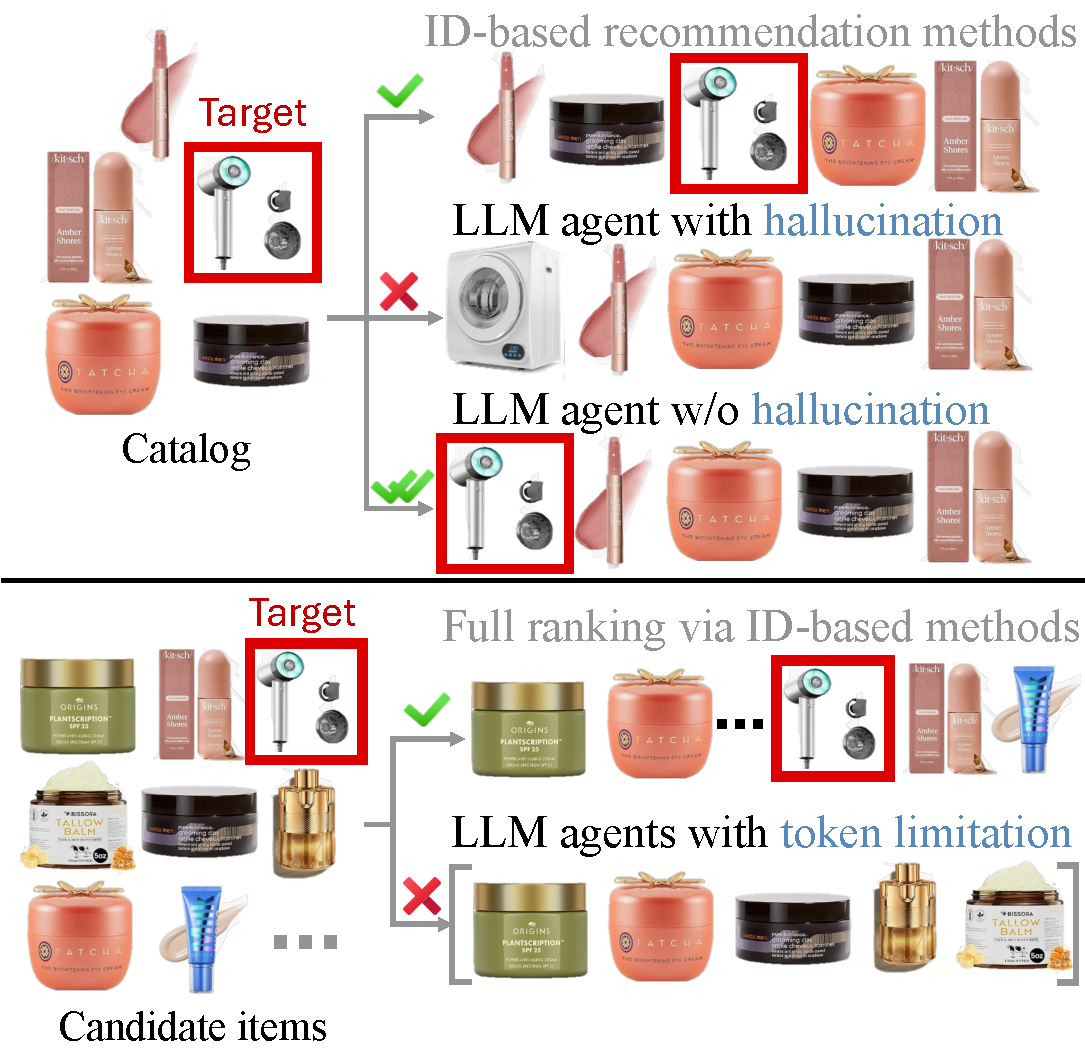
\includegraphics[scale=0.5]{sections/6_AgentDR/figures/motivation/motivation.pdf}
    \caption{Two challenges in directly deploying LLMs for recommendation.}
    \label{fig_agentdr:motiv}
\end{figure}

Given the limitations of using LLMs solely as feature encoders or standalone recommenders, recent studies have investigated leveraging LLMs as interactive agents for recommendation~\cite{agentcf, agent4rec, recagent}. Rather than relying only on direct prompting with user interaction histories, these agent-based approaches integrate memory modules to preserve long-term context and better harness collaborative signals throughout the recommendation process. 
% During training, the agent memories are dynamically updated based on observed behavioral patterns through a reflection mechanism, allowing the agent to iteratively refine its internal representation of user preferences. 
While LLM-based agents alleviate the representational constraints of static numerical embeddings and enable adaptive modeling of user behavior over time, they also inherit key limitations from the generative nature of LLMs. As illustrated in Fig.~\ref{fig_agentdr:motiv}, two primary drawbacks arise in previous agent-based works when directly applying LLMs for recommendation: (i) the tendency to hallucinate non-existent items that are not part of the product catalog, and (ii) the high inference cost and token length constraints, which make them impractical for large-scale item ranking. Moreover, longer input and output sequences further increase the risk of hallucination due to attention bottlenecks and heightened generation uncertainty~\cite{hallulength1}.

As a result, when applied to recommendation scenarios, existing LLM-based agents~\cite{agentcf, iagent, agent4rec} typically evaluate performance by checking whether the ground-truth item, which is the next item that the user actually interacted, is correctly ranked against a small set of negative candidates. These negative candidates are items randomly sampled from the catalog that the user did not interact with during the observation window, serving as distractors in the ranking process. However, this setup is fundamentally misaligned with most real-world recommendation scenarios, where systems must select the most relevant items from massive catalogs that often contain thousands of items. Restricting the candidate set to such a small range can artificially inflate performance, overlook the complexity of large-scale ranking, and hinder the system’s ability to identify truly relevant items in open-ended domains.

Besides their limitations in full-ranking, previous LLM-based agents primarily focus on modeling user preferences from explicit user-item interactions, which already can be effectively modeled by traditional embedding-based recommendation methods~\cite{simplex, enmf, LightGCN}. On the contrary, traditional models often overlook higher-level semantic relations between items that go beyond co-occurrence patterns. 
To address this gap, the generative capabilities and extensive world knowledge of LLMs make them particularly well-suited for reasoning over implicit relationships, such as complementarity and substitution relations.
Substitutes help identify alternative options when a preferred item is unavailable or when the user seeks variety, while complements reveal co-purchase patterns that often indicate planned or contextual consumption behaviors. 
For example, a user purchasing a digital single-lens reflex camera often requires a tripod as a complement, whereas a user who buys tiramisu is more likely to choose cheesecake as substitute over burgers when the original item is out of stock.
Although such relationships can greatly enhance recommendation quality~\cite{subcom22, subcom23, Nerrise25-substitution}, the ground-truth labels of them are typically absent from most datasets~\cite{dataset:amazon, xmarket}. Furthermore, annotating item pairs with accurate relational labels often requires extensive world knowledge and nuanced understanding, making manual annotation both expensive and time-consuming. This gap highlights the potential of LLMs as an alternative source of relational knowledge. By leveraging their extensive pretraining on diverse textual data, LLMs can capture subtle functional relationships between items, enabling automatic discovery of substitutes and complements that would otherwise require labor-intensive human annotation.

Considering the two issues discussed above, we propose a novel LLM-based agent framework that leverages the complementary strengths of LLMs and traditional recommendation models. This framework addresses hallucination by grounding all recommendations in catalog-aware models. The reasoning ability and world knowledge of LLMs are utilized to integrate the ranking results of multiple recommendation tools and to perform fine-grained refinement of the combined ranking results, both in a personalized manner. For each user, an agent is optimized to assess the suitability of each recommendation tool by measuring the gap between the tool’s outputs and the user’s true preferences. In parallel, the user’s intent to purchase substitutes or complements is inferred by the LLM based on the user’s historical behavior. During inference, the agent first leverages the stored tool suitability to integrate the outputs from all tools, and then applies the inferred user intent to refine the combined ranking results.
Building on this framework, we highlight the main contributions of our work as follows:
\begin{itemize}[left=0pt]
    \item \textbf{Novel Framework.} We propose an agent-based framework AgentDR, where LLM-based agents delegate full-ranking recommendation to recommendation tools that excel at modeling complex user behavior patterns. This separation enables the integration of the scalability and efficiency of traditional recommenders with the reasoning capabilities of LLMs.
    \item \textbf{Item-item Reasoning.} We leverage the world knowledge of LLMs for implicit item-item relationship reasoning to enhance recommendation. Each user agent generates substitute and complement candidates based on the user's historical preferences, and accordingly refines recommendation results.
    \item \textbf{Comprehensive Evaluation.} Extensive experiments verify the effectiveness of our approach in full-ranking performance on three public datasets. Besides recall and NDCG, we propose a LLM-based metric to jointly assess the semantic relevance and ordering correctness of the predicted ranking lists.
\end{itemize}

\section{Related Works}

\begin{table}
\centering
\resizebox{0.8\textwidth}{!}{%
\begin{tabular}{l c c c}
\toprule
%Method
& Full Ranking
& Text Feature
& Generative  \\
& Evaluation
& Handling
& Reasoning\\
\midrule
Recommender based on interactions
& \cmark & \xmark & \xmark \\
LLM as Encoder
& \cmark & \cmark & \xmark \\
LLM as Recommender
& \xmark & \cmark & \cmark \\
LLM-Rec Agents~\cite{interecagent, recmind, agentcf, agent4rec, recagent, iagent}
& \xmark & \cmark & \cmark \\
\midrule
AgentDR
& \cmark & \cmark & \cmark \\
\bottomrule
\end{tabular}%
}
\caption{Comparison of AgentDR and other recommendation methods.}
\label{tab_agentdr:salesman}
\end{table}


LLM-based agents have recently demonstrated strong capabilities in using memory and reflection to learn from past experiences and simulate human-like behaviors~\cite{gao2025, ZhongGGYW24, ShinnCGNY23, ZhaoTZC024, ShiJQY24, LiDWCF24}. In the context of recommendation, LLM-based agents have been used to investigate social phenomena such as information cocoons and filter bubble effect by simulating user behaviors~\cite{recagent, agent4rec}.
%Agent4Rec~\cite{agent4rec} reproduces the filter bubble effect and uncovers its underlying causal mechanisms. 
Given that agent-based frameworks can offer deeper insights into user behavior by leveraging the reasoning capabilities of LLMs, there is a growing interest in applying LLM-based agents to enhance recommendation performance~\cite{recmind, interecagent, agentcf, iagent}. 
% RecMind~\cite{recmind} leverages historical data to build user agents for few-shot recommendation. InteRecAgent~\cite{interecagent} connects LLM capabilities with tools for conversational recommendation. AgentCF~\cite{agentcf} employs collaborative reflection to update memory of both user and item agents. User instructions and reviews are also leveraged to flexibly express user preferences beyond just product attributes in iAgent~\cite{iagent}.
Nonetheless, since hallucination~\cite{hallu1, hallu2} and token limitation remain two challenges when applying these agents to rank all items in the datasets for each user, most prior works~\cite{agentcf, recmind, interecagent, agent4rec, recagent, iagent} lack of full-ranking ability. The batch-ranking task in these works is fundamentally misaligned with most real-world scenarios, where RecSys are required to rank relevant items from massive catalogs. And these works focus on predicting user behaviors based on user-item interactions, a signal that traditional recommendation models~\cite{LightGCN, sasrec, simplex} are already well-equipped to capture and exploit. Different from these works, our framework combines the strengths of LLMs and traditional recommenders to achieve personalized full-ranking. Comparison between different approaches is summarized in Table~\ref{tab_agentdr:salesman}.


\section{Proposed Framework: AgentDR}

\begin{figure*}[]
    \centering
    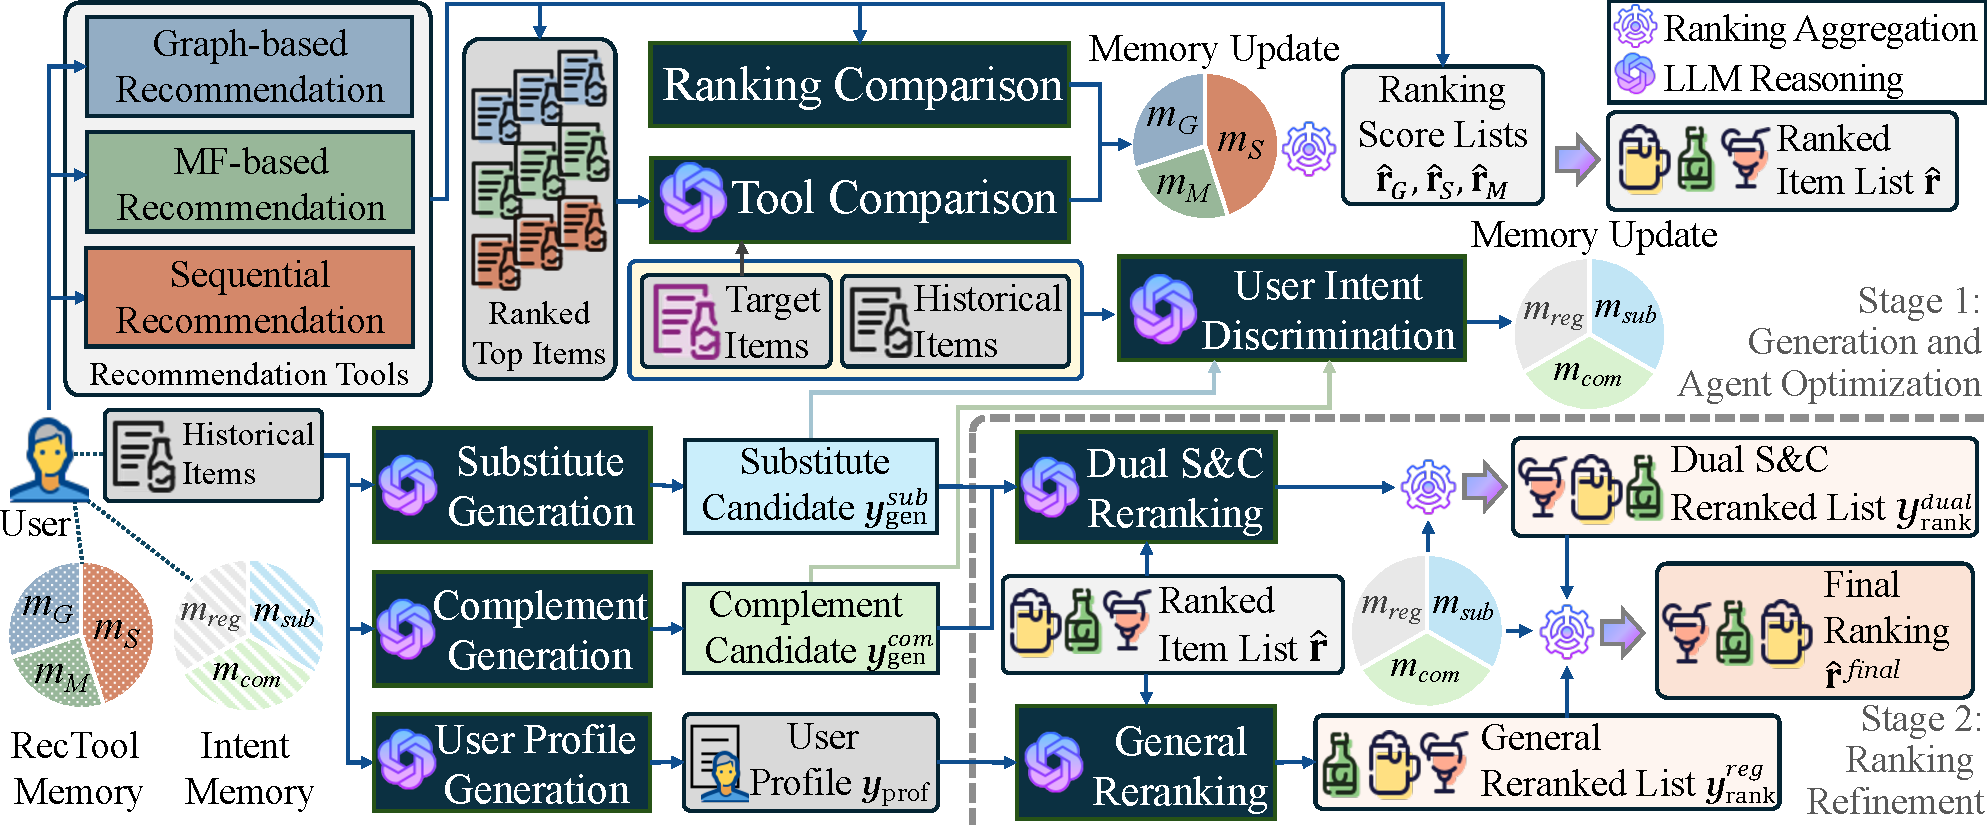
\includegraphics[scale=0.48]{sections/6_AgentDR/figures/framework3.pdf}
    \caption{The framework of AgentDR.
    % : Each user agent is equipped with two memory modules: RecTool memory to store tool suitability, and intent memory to track user intent. Ranking results from recommendation tools are aggregated based on RecTool memory. The aggregated result is further refined by the dual S\&C and general ranking modules.
    }\label{fig_agentdr:framework}
\end{figure*}

\subsection{Preliminaries}
\subsubsection{Problem Formulation}
Let $\mathcal{I}$ and $\mathcal{U}$ denote the complete item pool and the set of users in the dataset, respectively. Specifically, each user $u \in \mathcal{U}$ is associated with a behavior sequence $\mathbf{s} = (i_1, i_2, \dots, i_n)$, where $i_j \in \mathcal{I}$ denotes the $j$-th item interacted with by user $u$. Furthermore, each item $i \in \mathcal{I}$ is accompanied by its corresponding textual description. For simplicity, we use $\text{desc}(\mathbf{s})$ to denote the list of textual descriptions for all items from item sequences $\mathbf{s}$.
Given a user's historical interaction sequence $\mathbf{s}_{[:-k]}$ and the corresponding item description list, the goal is to predict the next item $i_{k+1} \in \mathcal{I}$ that the user is likely to interact with. 
This is commonly framed as a ranking task: each user agent is expected to assign higher scores to items that better match the user's preferences, as inferred from both behavioral patterns and textual semantics. The final output is a ranked list of $\mathcal{I}$ tailored to this user $u$. For clarity, the subscript $u$ will be omitted in subsequent sections, given that each user agent functions independently.

\subsubsection{Recommendation Tools}~\label{sec:rectools}
AgentDR is an agent-based framework compatible with different recommendation methods as tools under the minimal assumption that they produce a full-ranking list of items. These recommendation methods are treated as tools and collectively form the tool set $\mathcal{T}$. For a broad coverage of recommendation modeling strategies, we utilize three types of recommendation tools to perform recommendation tasks within AgentDR: (i) a graph-based model with output ranking score list $\hat{\mathbf{r}}_{G}$; (ii) a sequential recommendation model with output ranking score list $\hat{\mathbf{r}}_{S}\in\mathbb{R}$; and (iii) a MF-based model with output ranking score list $\hat{\mathbf{r}}_{M}$. All these output lists are in $\mathbb{R}^{1\times|\mathcal{I}|}$. The three model instances used in this work are elaborated in Sec.~\ref{sec:toolselect}. These models are pretrained on the first $(n-k)$ items, denoted as $\mathbf{s}_{[:-k]}$.

\subsubsection{Framework Overview} The overall framework of AgentDR is depicted in Fig.~\ref{fig_agentdr:framework}. Each user agent is equipped with a profile and two memory modules (Sec.~\ref{sec:profile_mem}). 
% The agent memory is optimized in the first stage and then used for ranking refinement in the second stage. 
The agent optimization begins with prompting the LLM to generate potential substitutes and complements for each user (Sec.~\ref{sec:scgen}). Next, the agent memory is optimized by distinct reflection mechanisms. The RecTool memory is optimized through personalized tool selection (Sec.~\ref{sec_tool_select}), while the intent memory is optimized via user intent discrimination (Sec.~\ref{sec:intent_compare}). Finally, the top items from the aggregated rankings of multiple tools are refined by dual S\&C reranking module (Sec.~\ref{sec:dualrerank}).

\subsection{User Profile and Memory}\label{sec:profile_mem}
\subsubsection{User Profile Summarization}~\label{sec:userprof}
Explicit user profiles are usually unavailable in most public real-world datasets. Thus, we summarize the user profile from users' historical interactions by leveraging the reasoning capabilities and world knowledge of LLMs. To be concrete, we prompt the LLM to summarize the user's preference from descriptions of historical items for each user. And this preference is used as the user profile $p$ of each user agent:
\begin{equation}\label{eq_agentdr:gen_prof}
        y_{\text{prof}} = \text{LLM}_\text{prof}(\text{desc}(\mathbf{s})),
\end{equation}
where $\text{LLM}_\text{prof}(\cdot)$ represents the LLM prompted to transform these texts into a coherent user profile. Due to limited space, the details of all prompts used in AgentDR are shown in Appendix~\ref{app:prompts}.

\subsubsection{User Agent Memory}
In contrast to static user profiles, memories are employed to enable user agents to dynamically maintain context in response to agent optimization based on consecutive user behaviors. 
% The relationship between user profiles and agent memory is analogous to the distinction between fixed one-hot feature vectors and trainable embeddings in traditional models. 
We equip each user agent with two compact memory modules: \textit{RecTool} memory and \textit{intent} memory. RecTool memory $\mathbf{m}^{rec}\in\mathbb{R}^{1\times |\mathcal{T}|}$ is a list of weights reflecting the suitability of each recommendation tool for each user, where $|\mathcal{T}|$ is the number of recommendation tools. For LightGCN, SASRec and SimpleX deployed in this paper, we denote their weights in memory as $m_G$, $m_S$ and $m_M$, respectively. Similarly, intent memory $\mathbf{m}^{int}\in\mathbb{R}^{1\times 3}$ contains three weights $m_{sub}$, $m_{com}$ and $m_{reg}$ , denoting the user's intent toward substitutes, complements, and other regular items, respectively. In AgentDR, RecTool memory is optimized by tool comparison and ranking comparison modules, detailed in Sec.~\ref{sec:tool_compare} and~\ref{sec:rank_compare}. Intent memory is optimized by a intent discrimination module in Sec.~\ref{sec:intent_compare}.

\subsection{Substitute and Complement Generation}~\label{sec:scgen}
A key challenge in enhancing personalization through substitution and complementarity is that such relationships are usually implicit in most datasets. Annotating these pairwise relationships with LLMs across a large number of items demands substantial computational resource, as it involves $\mathcal{O}(|\mathcal{I}|^2)$ LLM inference calls. To mitigate computational overhead, AgentDR is designed to refine the top-ranked items from recommendation tools based on the substitutes and complements of the user’s latest preferences. The first step in this process involves generating potential substitutes and complements based on the user’s historical behaviors. Specifically, we prompt the LLM to generate a list of substitutes and a list of complements corresponding to the user’s recent interests:
\begin{align}
    y_{\text{gen}}^{sub} &= \text{LLM}_\text{gen}^{sub}(\text{desc}(\mathbf{s}_{[-(k+c):-k]})) \label{eq_agentdr:gen_sub}\\
    y_{\text{gen}}^{com} &= \text{LLM}_\text{gen}^{com}(\text{desc}(\mathbf{s}_{[-(k+c):-k]})), \label{eq_agentdr:gen_com}
\end{align}
where $\mathbf{s}_{[-(k+c):-k]}$ denotes the most recent $c$ items visible to the recommendation tools in the sequence. The textual outputs $y_{\text{gen}}^{sub}$ and $y_{\text{gen}}^{com}$ represent the generated lists of substitutes and complements, each of length $c$. The functions $\text{LLM}_\text{gen}^{sub}(\cdot)$ and $\text{LLM}_\text{gen}^{com}(\cdot)$ denote the prompt functions for generating substitutes and complements, respectively.
From a complexity perspective, we reduce the LLM inference calls from $\mathcal{O}(|\mathcal{I}|^2)$ for pairwise annotation to $\mathcal{O}(|\mathcal{U}|)$ for personalized intent generation. This reduction substantially enhances scalability in real-world scenarios, such as online grocery involving millions of items.


\subsection{Personalized Tool Selection}~\label{sec_tool_select}
\subsubsection{LLM-based Tool Comparison}~\label{sec:tool_compare}
Different users exhibit distinct behavior patterns and therefore benefit from different recommendation strategies. For instance, users who read books like \textit{Harry Potter} often proceed with its sequels, making sequential recommendation models particularly effective. After finishing all the sequels, users may be interested in other fictions read by similar users, where collaborative filtering proves more suitable. To enable personalized tool selection for each user, AgentDR incorporates a tool comparison module that performs a holistic evaluation across multiple recommendation tools. In this module, the user agent is tasked with identifying the best tool based on recommended results of tools and ground-truth user preference:
\begin{equation}~\label{eq_agentdr:tool_cmpr}
    \mathbf{z}_{\text{cpr}} = \text{LLM}_{\text{cpr}}(\{\text{desc}(f_\text{top}(\hat{\mathbf{r}}_{t}, k_{\text{cpr}}))|t\in \mathcal{T}\}, \text{desc}(\mathbf{s}_{[-k:]})),
\end{equation}
where the output $\mathbf{z}_{\text{cpr}}$ consists of $|\mathcal{T}|$ binary indicators, each indicating whether tool $t$ provides the most relevant recommendation to the user's preference among all tools in $\mathcal{T}$. For instance, $z_{\text{cpr}}^{G} = 1$ indicates that the LLM has selected the graph-based tool as the best match to the user’s preferences.
We use $f_\text{top}(\hat{\mathbf{r}}_{t}, k_{\text{cpr}})$ to represent the sequence of top-$k_{\text{cpr}}$ items ranked by recommendation tool $t$. Subsequence $\mathbf{s}_{[-k:]}$ refers to the most recent $k$ user-interacted items, which are withheld from training of recommendation tools and used as ground-truth signals to optimize the agent's decision-making. The function $\text{LLM}_\text{cpr}(\cdot)$ is used to prompt the LLM to compare the input sequences and select the tool most aligned with the user's preferences.
After the LLM identifies the tool that best aligns with the user’s recent preferences, the tool weight $m_{t}\in \{m_G, m_S, m_M\}$ in RecTool memory is updated accordingly:
\begin{equation}\label{eq_agentdr:toolcpr}
    m_{t} \leftarrow  m_{t} + \alpha\cdot z_{\text{cpr}}^{t}, 
\end{equation}
where $\alpha$ is the learning rate to update RecTool memory by this module. 
This tool comparison remains robust even when multiple tools appear effective. It addresses two key challenges: LLMs tend to agree with any reasonable recommendation, and single-domain datasets often make all outputs appear relevant.

\subsubsection{Ranking Comparison and Aggregation}~\label{sec:rank_compare}
Besides the LLM-based tool comparison, we also compare the ranking performance based on the ranks of the most recent $k$ items in each tool:
\begin{equation}~\label{eq_agentdr:rankcmpr}
    m_{t} \leftarrow  m_{t} + \beta\sum_{\{r^j_{t}|i_j\in\mathbf{s}_{[-k:]}\}}\frac{(r^j_{t})^{-1}}{\sum_{t'\in\mathcal{T}}(r^j_{t'})^{-1}},
\end{equation}
where $r^j_{t}$ is the rank of the $j$-th item from tool $t$.
This quantitative comparison yields a behavior-grounded signal reflecting how well each tool generalizes to unseen user preferences in $\mathbf{s}_{[-k:]}$. 
To obtain a comprehensive ranked list from all tools, a weighted sum is computed based on the updated RecTool memory:
\begin{equation}~\label{eq_agentdr:aggrank}
    \hat{\mathbf{r}} = \sum_{t\in\mathcal{T}}m_t\hat{\mathbf{r}}_t = m_G\hat{\mathbf{r}}_{G} +m_S\hat{\mathbf{r}}_{S} + m_M\hat{\mathbf{r}}_{M},
\end{equation}
where $\hat{\mathbf{r}}\in\mathbb{R}^{1\times|\mathcal{I}|}$ is the aggregated ranked item list. This simple yet effective rank-level ensemble strategy allows the agent to adaptively combine tools based on user-specific preferences. It also remains flexible and can be replaced by more complex list-wise combination mechanisms based on backpropagation. We implement and compare different ensemble strategies for ranking comparison and aggregation in Sec.~\ref{sec:ensemble}.

\subsection{Intent Discrimination}~\label{sec:intent_compare}
Understanding whether a user’s next interaction is driven by substitutes, complements, or general interest is crucial for tailoring recommendations that match their intent. Traditional ID-based recommenders struggle to distinguish these patterns, as they require nuanced semantic and functional reasoning that goes beyond co-occurrence statistics. With reasoning ability of LLMs, user agents can allocate attention to the most relevant pathway while ensuring coverage of diverse user behaviors, ultimately improving ranking robustness and relevance.
\subsubsection{Substitution and Complementarity}
Based on implicit item-item relationships, we first distinguish the user's potential intent between substitutes and complements. Given the substitute list $y_{\text{gen}}^{sub}$ and the complement list $y_{\text{gen}}^{com}$ generated in Sec.~\ref{sec:scgen}, we prompt the LLM to access the user's interest in substitute or complements by comparing the generated lists with the ground-truth preferences:
\begin{equation}~\label{eq_agentdr:scdcm}
     \mathbf{z}_{\text{dcm}} = \text{LLM}_\text{dcm}(y_{\text{gen}}^{sub}, y_{\text{gen}}^{com}, \text{desc}(\mathbf{s}_{[-k:]})),
\end{equation}
where the output $\mathbf{z}_{\text{dcm}}$ consists of two binary indicators $z_{\text{dcm}}^{sub}$ and $z_{\text{dcm}}^{com}$, which sum to 1. Each indicator reflects whether the corresponding list exhibits greater semantic and functional alignment with the user's recent interactions. The function $\text{LLM}_\text{dcm}(\cdot)$ prompts the LLM to identify whether the substitute or complement list better matches the user’s recent preferences.

\subsubsection{General Interest}
In addition, a separate module is employed to assess the user's general interest in items other than substitutes or complements, based on the user’s historical behavior:
\begin{equation}\label{eq_agentdr:reglearn}
     z_{\text{dcm}}^{reg} = \text{LLM}_\text{dcm}^{reg}(\text{desc}(\mathbf{s})),
\end{equation}
where the output $z_{\text{dcm}}^{reg}$ of prompt function $\text{LLM}_\text{dcm}^{reg}(\cdot)$ is a binary indicator that equals 1 if the ground-truth user preferences do not exhibit clear substitute or complement patterns otherwise 0. This additional assessment ensures coverage of a broader spectrum of user behaviors, particularly in scenarios where the user’s preferences are not driven by substitution or complementarity. Identifying such general interest prevents the agent from overfitting to relational reasoning. This mitigates the risk of forcing item-item relational interpretations where they do not apply.

\subsubsection{General Reranking}\label{sec:genrerank}
To account for general interests of users, a reranking module is introduced to refine the recommendations based on the semantic similarity between the candidate items and the users' general preferences. For each user, the general preferences have been summarized from historical items as user profile in Sec.~\ref{sec:userprof}. Then the LLM is prompted to rerank the top items based on the user profile $y_{\text{prof}}$, denoted as function $\text{LLM}^{reg}_{\text{rank}}(\cdot)$:
\begin{equation}~\label{eq_agentdr:gen_rerank}
    y_{\text{rank}}^{reg} = \text{LLM}^{reg}_{\text{rank}}(f_\text{top}(\hat{\mathbf{r}},k'), \text{desc}(f_\text{top}(\hat{\mathbf{r}},k')),y_{\text{prof}}),
\end{equation}
where $f_\text{top}(\hat{\mathbf{r}},k')$ is the top $k'$ items in the aggregated ranked list $\hat{\mathbf{r}}$, and $y_{\text{rank}}^{reg}$ is the reranked list containing $k'$ item IDs.

\subsubsection{Intent Memory Update}
Similar to RecTool memory update in Eq.~\ref{eq_agentdr:toolcpr}, the corresponding intent $m_{int}\in \{m_{sub}, m_{com}, m_{reg}\}$ is updated based on $z_{\text{dcm}}^{int}\in \{z_{\text{dcm}}^{sub}, z_{\text{dcm}}^{com}, z_{\text{dcm}}^{reg}\}$ by a learning rate $\gamma$:
\begin{equation}\label{eq_agentdr:intentdcm}
    m_{int} \leftarrow  m_{int} + \gamma\cdot z_{\text{dcm}}^{int}.
\end{equation}
This intent discrimination module equips the agent with a nuanced understanding of user preferences, enabling it to adaptively allocate attention to different reasoning modes and thereby guide downstream reranking in a more personalized manner.

\subsection{Dual S\&C Reranking}\label{sec:dualrerank}
A dual substitute and complement (S\&C) reranking module is proposed to comprehensively refine the recommendation results from tools in AgentDR. First, to leverage substitute and complement relation reasoning to enhance recommendation via world knowledge of the LLM, we design two independent reranking modules to refine the top-ranked items based on their semantic similarity with the candidate substitutes and complements for a user:
\begin{align}
    y_{\text{rank}}^{sub} &= \text{LLM}_{\text{rank}}(f_\text{top}(\hat{\mathbf{r}},k'), \text{desc}(f_\text{top}(\hat{\mathbf{r}},k')),y_{\text{gen}}^{sub}) \label{eq_agentdr:rerank_sub}\\
    y_{\text{rank}}^{com} &= \text{LLM}_{\text{rank}}(f_\text{top}(\hat{\mathbf{r}},k'), \text{desc}(f_\text{top}(\hat{\mathbf{r}},k')),y_{\text{gen}}^{com}), \label{eq_agentdr:rerank_com}
\end{align}
where output $y_{\text{rank}}^{sub}$ and $y_{\text{rank}}^{com}$ are the reranked lists containing the same $k'$ items from $f_\text{top}(\hat{\mathbf{r}},k')$. The LLM is prompted to rerank the top items from the aggregated ranked list based on their similarity to candidate substitutes and complements, denoted as $\text{LLM}_{\text{rank}}(\cdot)$. 

Although the expected output of the reranked list is a sequence of exactly $k'$ item IDs selected from the ID-only list $f_\text{top}(\hat{\mathbf{r}},k')$, the LLM may hallucinate by generating invalid outputs such as non-existent item IDs or irrelevant text. To address this issue, we apply a rule-based hallucination filtering mechanism to ensure output validity. Specifically, only valid item IDs in the item corpus are retained in the reranked list. If the resulting list contains fewer than $k'$ items, the remaining valid IDs from $f_\text{top}(\hat{\mathbf{r}},k')$ are appended to the end of the valid list in original order. This filtering mechanism is also applied in the aforementioned general reranking.
% Compared to prior approaches that rely on carefully crafted query prompts or self-reflection mechanisms to mitigate hallucination~\cite{agentcf, agent4rec, iagent}, 
This strategy completely eliminates the impact of hallucination on the ranking task, while incurring minimal computational overhead and requiring minimal reliance on the LLM’s instruction-following capability.

Subsequently, to account for individual variation in user intent, we personalize the combination of the two reranked ID lists using a ranking fusion function $f_{\text{fuse}}(\cdot)$. This function takes the two ID lists and the corresponding intent weights as input:
\begin{equation}\label{eq_agentdr:fuse}
    \mathbf{\hat{r}}^{dual} = f_{\text{fuse}}((m_{sub}, y_{\text{rank}}^{sub}), ( m_{com}, y_{\text{rank}}^{com})),
\end{equation}
where the ranking score $\hat{r}_{i}^{dual}$ of each item $i$ in this output list $\mathbf{\hat{r}}^{dual}$ is computed as a weighted sum of the item's positions in the two input lists:
\begin{equation}
    \hat{r}_{i}^{dual} = m_{sub}\cdot\text{index}(i, y_{\text{rank}}^{sub}) + m_{com}\cdot\text{index}(i, y_{\text{rank}}^{com}), 
\end{equation}
where $\text{index}(i,\cdot)$ returns the rank position of item $i$ within a given list. This personalized fusion strategy allows the agent to balance substitute-based and complement-based reasoning in accordance with the inferred user intent, without incurring additional LLM inference overhead.
The output list $\mathbf{\hat{r}}^{dual}$ is further fused with the item list from general reranking:
\begin{equation}\label{eq_agentdr:regfuse}
    \mathbf{\hat{r}}^{final} = f_{\text{fuse}}((1, y_{\text{rank}}^{dual}), (m_{reg}, y_{\text{rank}}^{reg})),
\end{equation}
where $y_{\text{rank}}^{dual}$ denotes the item list sorted by ranking scores in $\mathbf{\hat{r}}^{dual}$. The final recommendation output consists of the top-$k'$ items ranked by their scores in $\mathbf{\hat{r}}^{final}$. By incorporating the broader user preference profile as a form of regularization in the reranking process, the agent achieves a more robust recommendation strategy, particularly when relational cues among items are weak or absent.


\subsection{Details of Prompts}\label{app:prompts} 
The detailed contents of prompts used in AgentDR are shown from Table~\ref{app:tab:gen_prof} to Table~\ref{app:tab:dualrerank}. 
%{\color{red} ** Do you want to add the prompts for VDCG evaluation too? we have room}

\begin{promptbox}
\small
\begin{tabularx}{\linewidth}{X}
\toprule
\textbf{[Instruction]}\\
Summarize the user's preference based on the historical items this user purchased under \emph{Electronics} on \emph{Amazon}.\\[0.4em]
\textbf{[Historical Items]}\\
\{item\_descriptions\}\\
\bottomrule
\end{tabularx}
\end{promptbox}
\captionof{table}{Prompts in AgentDR for $\text{LLM}_\text{prof}(\cdot)$.}
\label{app:tab:gen_prof}

% \medskip

\begin{promptbox}
\small
\begin{tabularx}{\linewidth}{X}
\toprule
\textbf{[Instruction]}\\
According to the historical items purchased by a user, generate \emph{20} \emph{substitutes} of these items under \emph{Electronics} on \emph{Amazon}.\\[0.4em]
\textbf{[Historical Items]}\\
\{item\_descriptions\}\\[0.4em]
The output must be one list of item titles in length of \emph{20}, separated by lines.\\
\bottomrule
\end{tabularx}
\end{promptbox}
\captionof{table}{Prompts in AgentDR for $\text{LLM}_\text{gen}^{sub}(\cdot)$.}
\label{app:tab:gen_subs}
% \medskip

\begin{promptbox}
\small
\begin{tabularx}{\linewidth}{X}
\toprule
\textbf{[Instruction]}\\
Under \emph{Electronics} on \emph{Amazon}, according to the descriptions of items in three groups A, B and C, evaluate which group the target item is most relevant to.\\[0.4em]
\textbf{[Group A]}\\
\{item\_descriptions\}\\[0.4em]
\textbf{[Group B]}\\
\{item\_descriptions\}\\[0.4em]
\textbf{[Group C]}\\
\{item\_descriptions\}\\[0.4em]
\textbf{[Target Item]}\\
\{target\_item\_description\}\\[0.4em]
The output must be one single character in \{A, B, C\} denoting the most relevant group.\\
\bottomrule
\end{tabularx}
\end{promptbox}
\captionof{table}{Prompts in AgentDR for $\text{LLM}_\text{cpr}(\cdot)$.}
\label{app:tab:cpr}
\medskip

\begin{promptbox}
\small
\begin{tabularx}{\linewidth}{X}
\toprule
\textbf{[Instruction]}\\
Given the two groups of items under \emph{Electronics} on \emph{Amazon}, evaluate which group is more relevant to the target item.\\[0.4em]
\textbf{[Group 1]}\\
\{item\_descriptions\}\\[0.4em]
\textbf{[Group 2]}\\
\{item\_descriptions\}\\[0.4em]
\textbf{[Target Item]}\\
\{target\_item\_description\}\\[0.4em]
The output must be one single number in \{1, 2\} denoting the more relevant group.\\
\bottomrule
\end{tabularx}
\end{promptbox}
\captionof{table}{Prompts in AgentDR for $\text{LLM}_\text{dcm}(\cdot)$.}
\label{app:tab:dcm}
\medskip

\begin{promptbox}
\small
\begin{tabularx}{\linewidth}{X}
\toprule
\textbf{[Instruction]}\\
According to the historical items purchased by a user under \emph{Electronics} on \emph{Amazon}, evaluate if this user exhibits clear substitute/complement patterns or not.\\[0.4em]
\textbf{[Historical Items]}\\
\{item\_descriptions\}\\[0.4em]
The output must be one single word in \{Yes, No\}.\\
\bottomrule
\end{tabularx}
\end{promptbox}
\captionof{table}{Prompts in AgentDR for $\text{LLM}_\text{dcm}^{reg}(\cdot)$.}
\label{app:tab:dcm_reg}
\medskip

\begin{promptbox}
\small
\begin{tabularx}{\linewidth}{X}
\toprule
\textbf{[Instruction]}\\
According to the user profile, rank top-\emph{20} items this user may prefer from the candidate item list, from higher to lower probability.\\[0.4em]
\textbf{[User Profile]}\\
\{user\_profile\}\\[0.4em]
\textbf{[Candidate Item List in format of (ID, description)]}\\
\{(item\_IDs, item\_descriptions)\}\\[0.4em]
The output must be a list of candidate item IDs with length of \emph{20}, with items separated by lines.\\
\bottomrule
\end{tabularx}
\end{promptbox}
\captionof{table}{Prompts in AgentDR for $\text{LLM}_\text{rank}^{reg}(\cdot)$.}
\label{app:tab:rank_reg}
\medskip

\begin{promptbox}
\small
\begin{tabularx}{\linewidth}{X}
\toprule
\textbf{[Instruction]}\\
Rank top-\emph{20} items from the candidate item list based on their similarity to the target item list, from higher to lower similarity.\\[0.4em]
\textbf{[Target Item List ordered by priority]}\\
\{item\_descriptions\}\\[0.4em]
\textbf{[Candidate Item List in format of (ID, description)]}\\
\{(item\_IDs, item\_descriptions)\}\\[0.4em]
The output must be a list of candidate item IDs with length of \emph{20}, with items separated by lines.\\
\bottomrule
\end{tabularx}
\end{promptbox}
\captionof{table}{Prompts in AgentDR for $\text{LLM}_\text{rank}^{sub}(\cdot)$ and $\text{LLM}_\text{rank}^{com}(\cdot)$.}
\label{app:tab:dualrerank}



\section{Experiment}
Through our extensive empirical analysis, we aim to address the following research questions. 
\begin{itemize}[left=0pt]
    \item \textbf{RQ1:} How does AgentDR perform in full-ranking recommendation compared to other baselines?
    \item \textbf{RQ2:} Does incorporating LLM-based reasoning modules improve the semantic alignment of recommended items with user intent?
    \item \textbf{RQ3:} How do different ranking aggregation strategies affect the performance of AgentDR?
    \item \textbf{RQ4:} What is the individual contribution of each LLM-based module in AgentDR?
\end{itemize}
\subsection{Experiment Settings}
\subsubsection{Datasets}
We conduct experiments on three datasets: Instacart~\cite{instacart}, %\footnote{https://www.kaggle.com/yasserh/datasets}, 
Electronics and Sports~\cite{xmarket}. %\footnote{https://xmrec.github.io/data/us/}. 
Electronics and Sports are two sub-datasets from public XMarket dataset~\cite{xmarket}.
The statistics are summarized in Table~\ref{tab_agentdr:datasets}. 
\begin{table}\resizebox{0.5\textwidth}{!}{
  \begin{tabular}{l c c c}
        \toprule
        % \hline
        % \hline
        \textbf{Dataset} & Instacart & Electronics & Sports \\
        \midrule
        \textbf{User \#} & 6,987 & 4,966 & 10,873\\

        \textbf{Item \#} & 2,108 & 14,635 & 4,306\\

        \textbf{Interaction \#} & 5,105,339 & 91,819 & 55,990\\
        \textbf{Density} & 34.663\% & 0.126\% & 0.120\% \\
        \bottomrule
        % \hline
  \end{tabular}}
  \caption{Statistics of datasets for AgentDR.}
  \label{tab_agentdr:datasets}
\end{table}
\subsubsection{Tool selection}\label{sec:toolselect}
In this work, three pretrained recommendation models are used as tools within AgentDR: 
\textbf{(1) LightGCN}~\cite{LightGCN}, \textbf{(2) SASRec}~\cite{sasrec}, and \textbf{(3) SimpleX}~\cite{simplex}.
% \begin{enumerate}[left=0pt, label=\textbf{(\arabic*)}]
%     \item \textbf{LightGCN}~\cite{LightGCN}. A graph-based collaborative filtering model that simplifies traditional graph convolution network by removing feature transformations and nonlinearities.
%     % Same as matrix factorization (MF), its space complexity is $O((|\mathcal{I}|+|\mathcal{U}|)\cdot d)$ and time complexity is $O(L\cdot|E|\cdot d)$, where $L$ is the number of graph convolution layers, $|E|$ is the number of interactions and $d$ is the embedding size.
%     \item \textbf{SASRec}~\cite{sasrec}.  A sequential recommendation model based on Transformer, which captures the user's dynamic preferences by modeling the dependencies between historical items.
%     % Its space complexity is $O(|I|\cdot d + n\cdot d + d)$ and time complexity is $O(|\mathcal{U}|\cdot (n^2\cdot d+n\cdot d^2))$ per taining epoch, where $n$ is the length of behavior sequences.
%     \item \textbf{SimpleX}~\cite{simplex}. A MF-based model where a margin is applied to filter uninformative negative samples in the loss.
%     % It has the same space complexity with MF. The time complexity is $O(|E|\cdot (n+\overline{n})\cdot d)$ where $\overline{n}$ is the number of negative samples per interaction. 
% \end{enumerate}
The simplicity of these tools allows us to validate the effectiveness of our framework without relying on complex architectures, aligning with our goal of maintaining a model-agnostic design.
\subsubsection{Baselines}
Besides the individual recommendation tools, we compare AgentDR with eight other baselines.
First, other representative MF-based, diffusion-based, and sequential models are used as tradition recommendation baselines:
\begin{enumerate}[left=0pt, label=\textbf{(\arabic*)}, start=4]
    \item \textbf{ENMF}~\cite{enmf} introduces mathematical optimization that enable efficient full-data MF without negative sampling.
    \item \textbf{DiffRec}~\cite{diffrec} is a diffusion-based recommendation model that generates user interactions in a denoising manner.
    \item \textbf{FEARec}~\cite{fearec} enhances self-attention with frequency-aware mechanisms to capture high-frequency signals and periodic patterns for sequential recommendation.
\end{enumerate}
Both tools and recommendation baselines are pretrained on the first $(n-k)$ items of each user’s interaction sequence $\mathbf{s}_{[:-k]}$, following the standard training protocol of sequential recommendation for fair performance comparison.
% Since AgentDR is complementary to the existing full-ranking models and aims to enhance their recommendations via the reasoning capabilities and world knowledge of LLMs, further comparison with other individual recommendation models is left for future work. 
Following the previous works~\cite{agentcf, iagent}, we also compare AgentDR with language-based approaches:
\begin{enumerate}[left=0pt, label=\textbf{(\arabic*)}, start=7]
    \item \textbf{BM25}~\cite{bm25} ranks candidates according to their textual similarity with user historical interactions.
    \item \textbf{LLMRanker}~\cite{llmrank} uses the LLM as a zero-shot ranker, considering user sequential interaction histories as conditions.
\end{enumerate}
In addition to these language-based baselines, 
we compare AgentDR against recommendation tools integrated with Retrieval-Augmented Generation (RAG). 
Specifically, the LLM is prompted to generate the top 20 items from the 50 candidates retrieved by each tool, 
conditioned on the user’s behavior sequence. 
The same hallucination filtering mechanism from Sec.~\ref{sec:dualrerank} is applied for fair comparison. 
These baselines are represented as \textbf{(9)-(11) \boldmath RAG$_{\mathit{G/S/M}}$} for LightGCN, SASRec and SimpleX, respectively. 
Since most prior LLM-agent works~\cite{agentcf, recmind, interecagent, agent4rec, recagent, iagent} are unable to rank all items in datasets, we exclude them from the comparison table instead of reporting trivially low full-ranking performance.
\subsubsection{Evaluation Metrics}
Recall@\{10,20\} and NDCG@\{10,20\} are adopted for ranking performance evaluation. Additionally, we propose a novel metric that measures the semantic vicinity of the predicted item list to the ground-truth item in the following Sec.~\ref{sec:vdcg}.

\subsubsection{Implementation Details}
Since most item titles in the three grocery datasets used in experiments are self-explainable, we use titles as textual descriptions of items and remove all the items without titles. For each dataset, users' interactions are chronologically organized based on timestamps to construct user behavior sequences. Since our framework delegates full-ranking sequential recommendation tasks to existing models, we follow the same data preprocessing strategy in previous works~\cite{LightGCN, sasrec, simplex} to remove cold-start users and items.

The recommendation tools are pretrained on the first $(n-k)$ items of each user’s interaction sequence $\mathbf{s}_{[:-k]}$, following the standard training protocol in recommendation where models learn from early interactions and are evaluated on their ability to predict future behaviors. This setup ensures consistency across tools and enables fair performance comparison between our framework and other recommendation baselines.
A grid search is applied for searching learning rates $\alpha, \beta$ and $\gamma$ in \{1e-3, 5e-3, 1e-2, 5e-2, 1e-1\}. 
To mitigate overfitting, each learning rate is multiplied by a decay factor of 0.8 after every optimization epoch. The number of historical items $c$ used for substitute and complement generation is set to 10. Following the training scheme in sequential recommendation, the number of target items $k$ is set to 1 during optimization. Since the evaluation metrics consider at most top 20 items, the number of reranking candidates $k'$ is fixed at 20. All experiments are conducted using the Phi-4 language model, deployed locally with vLLM on eight Tesla V100 GPUs, each with 32 GB of VRAM. The temperature is set to 0 to ensure deterministic outputs.
Aside from the complexity of the recommendation tools described in Sec.~\ref{sec:rectools}, the quantized version of a single Phi-4 model requires less than 12 GB of VRAM. Following prior LLM-agent works~\cite{agentcf, recagent, interecagent}, we train the recommendation tools on the entire training set, and randomly sample 160 agents for optimization on each dataset.

\subsection{Cost Analysis}
The total LLM API calls in AgentDR consist of three parts: generation, agent optimization, and reranking. 
Generation (Eq.~\ref{eq_agentdr:gen_prof}, Eq.~\ref{eq_agentdr:gen_sub} and Eq.~\ref{eq_agentdr:gen_com})
and reranking (Eq.~\ref{eq_agentdr:gen_rerank}, Eq.~\ref{eq_agentdr:rerank_sub}, and Eq.~\ref{eq_agentdr:rerank_com}) contain 6 calls per user. 
Each epoch in agent optimization contains 3 calls (Eq.~\ref{eq_agentdr:tool_cmpr}, Eq.~\ref{eq_agentdr:scdcm} and Eq.~\ref{eq_agentdr:intentdcm}) per user.
Hence, the total number of calls is $6n + 3nt$ where $n$ and $t$ are the numbers of users and epochs, respectively.
With all the agent memory updated, AgentDR takes less than 1 second to generate the final ranking list for each user.
We acknowledge that LLM-based agents generally have higher inference latency than embedding-based recommendation models, but they are still practical for offline ranking or secondary-stage recommendation pipelines.

\subsection{Semantic Vicinity Evaluation: VDCG}~\label{sec:vdcg}
Unlike ID-based recommenders, language-based methods prioritize semantic similarity over behavioral patterns. As a result, the item lists they generate may better reflect a user’s interests, even if the exact target items are absent. For example, for a user interested in a black baseball helmet, a list of baseball helmets in other colors is clearly more relevant than a list of bicycle helmets, despite both yielding zero recall and NDCG. To better capture the semantic vicinity to the user intent, we propose a new LLM-based evaluation metric, Vicinity-DCG (VDCG), which jointly assesses the semantic alignment and ranking correctness of the predicted item list.

\begin{promptbox}
\small
\begin{tabularx}{\linewidth}{X}
\toprule
\textbf{[Instruction]}\\
Given the same category, rate how well each item from the recommended list matches the target item based on relevance, usefulness, and user interest.\\[0.4em]
\textbf{[Category]}\\
\{item\_category\}\\[0.4em]
\textbf{[Target Item]}\\
\{item\_description\}\\[0.4em]
\textbf{[Recommended List]}\\
\{item\_descriptions\}\\[0.4em]
The output must be a list of integers. Each score must be between 0 (very unrelated) and 9 (exact match).\\
\bottomrule
\end{tabularx}
\end{promptbox}
\captionof{table}{Prompts in AgentDR for VDCG evaluation.}
\label{app:tab:vdcg}

Specifically, we prompt the LLM to rate how well each item in the recommended list aligns with the ground-truth item in terms of relevance, usefulness, and user interest. The rating scale ranges from 0 to 9, where 0 indicates an entirely unrelated item, and 9 represents a perfect semantic match between the item descriptions. The prompts for VDCG evaluation is shown in Table~\ref{app:tab:vdcg}.
These ratings are treated as relevance scores to compute the DCG~\cite{dcg} for the list. For normalization, we divide by a customized ideal DCG, calculated from a synthetic ideal list of scores: $[p, p/2, ..., p/2^l]$, where $p$ is the maximum relevance score minus 1, and 
$l$ is the length of the list. This ideal score distribution reflects the empirical tendency of the LLM to assign higher scores to only a few semantic-related items, following an approximately exponential decay. VDCG thus captures both the semantic vicinity and ranking quality of the predicted list with respect to the user's true intent.

\subsection{RQ1: Ranking Performance Comparison}

\begin{table*}[]
\resizebox{\textwidth}{!}{%
\begin{tabular}{l rrrr @{\hspace{1.5em}} rrrr @{\hspace{1.5em}} rrrr}
\toprule
%Dataset
& \multicolumn{4}{c}{Instacart}
& \multicolumn{4}{c}{Electronics}
& \multicolumn{4}{c}{Sports} \\
\cmidrule(lr){2-5}\cmidrule(lr){6-9}\cmidrule(lr){10-13}
%Metric
& R@10 & R@20 & N@10 & N@20
& R@10 & R@20 & N@10 & N@20
& R@10 & R@20 & N@10 & N@20 \\
\midrule
LightGCN  & 0.0500 & 0.1188 & 0.0221 & 0.0398 & 0.1188 & 0.1313 & 0.0734 & 0.0765 & \uline{0.1438} & 0.1625 & 0.0997 & 0.1040 \\
SASRec    & 0.0875 & 0.1500 & 0.0395 & 0.0552 & 0.1188 & 0.1313 & 0.0635 & 0.0667 & 0.1000         & 0.1438 & 0.0554 & 0.0667 \\
SimpleX   & 0.0313 & 0.0500 & 0.0180 & 0.0226 & 0.1000 & 0.1063 & 0.0761 & 0.0776 & 0.1375         & 0.1563 & 0.0951 & 0.0999 \\
\midrule
ENMF      & 0.1125 & 0.1750 & 0.0711 & 0.0797 & 0.1250 & 0.1312 & 0.0881 & 0.0897 & 0.1375         & 0.1438 & \uline{0.1172} & \uline{0.1187} \\
DiffRec   & \uline{0.1188} & 0.1563 & \uline{0.0773} & 0.0806 & \uline{0.1562} & \uline{0.1688} & \uline{0.0971} & \uline{0.0981} & 0.1125 & 0.1188 & 0.0875 & 0.0890 \\
FEARec    & 0.1063 & \uline{0.1875} & 0.0639 & \uline{0.0845} & 0.1250 & 0.1625 & 0.0627 & 0.0726 & 0.1313 & 0.1563 & 0.0732 & 0.0797 \\
\midrule
BM25      & 0.0625 & 0.0875 & 0.0310 & 0.0370 & 0.1000 & 0.1313 & 0.0432 & 0.0514 & 0.1188 & 0.1250 & 0.0536 & 0.0552 \\
LLMRank   & 0.0750 & 0.1000 & 0.0373 & 0.0436 & 0.1000 & 0.1250 & 0.0503 & 0.0565 & 0.0938 & 0.1063 & 0.0458 & 0.0488 \\
\midrule
RAG$_G$   & 0.1125 & 0.1563 & 0.0480 & 0.0594 & 0.1125 & 0.1438 & 0.0715 & 0.0748 & 0.1125 & 0.1188 & 0.0750 & 0.0768 \\
RAG$_S$   & 0.0688 & 0.1063 & 0.0312 & 0.0405 & 0.1063 & 0.1188 & 0.0575 & 0.0605 & 0.1375 & \uline{0.1625} & 0.0852 & 0.0913 \\
RAG$_M$   & 0.0750 & 0.1125 & 0.0335 & 0.0427 & 0.0875 & 0.1250 & 0.0517 & 0.0613 & 0.1125 & 0.1375 & 0.0823 & 0.0871 \\
\midrule
AgentDR & \textbf{0.1563} & \textbf{0.2000} & \textbf{0.0796} & \textbf{0.0907}
          & \textbf{0.1688} & \textbf{0.2000} & \textbf{0.1180} & \textbf{0.1260}
          & \textbf{0.1750} & \textbf{0.2063} & \textbf{0.1247} & \textbf{0.1326} \\
Improv.   & 33.50\% & 6.67\% & 2.98\% & 7.34\%
          & 8.07\%  & 18.48\% & 21.52\% & 28.44\%
          & 21.67\% & 26.95\% & 6.40\% & 11.71\% \\
\bottomrule
\end{tabular}%
}\caption{Overall performance comparison of AgentDR with baselines.}\label{tab_agentdr:overall}
\end{table*}

% previous version
% \vspace{-3mm}
% \resizebox{0.9\textwidth}{!}{
% \begin{tabular}{l|rrrr|rrrr|rrrr}
% \hline
% % \hline
% Dataset    & \multicolumn{4}{c|}{Instacart}                                                                                         & \multicolumn{4}{c|}{Electronics}                                                                                            & \multicolumn{4}{c}{Sports}                                                                                           \\ \hline
% Metric     & \multicolumn{1}{c}{R@10}     & \multicolumn{1}{c}{R@20}    & \multicolumn{1}{c}{N@10}     & \multicolumn{1}{c|}{N@20}    & \multicolumn{1}{c}{R@10}     & \multicolumn{1}{c}{R@20}    & \multicolumn{1}{c}{N@10}     & \multicolumn{1}{c|}{N@20}    & \multicolumn{1}{c}{R@10}     & \multicolumn{1}{c}{R@20}    & \multicolumn{1}{c}{N@10}      & \multicolumn{1}{c}{N@20}     \\ \hline
% LightGCN & 0.0500 & 0.1188 & 0.0221 & 0.0398 & 0.1188 & 0.1313 & 0.0734 & 0.0765 & \uline{0.1438} & 0.1625 & 0.0997 & 0.1040 \\
% SASRec & 0.0875 & 0.1500 & 0.0395 & 0.0552 & 0.1188 & 0.1313 & 0.0635 & 0.0667 & 0.1000 & 0.1438 & 0.0554 & 0.0667 \\
% SimpleX & 0.0313 & 0.0500 & 0.0180 & 0.0226 & 0.1000 & 0.1063 & 0.0761 & 0.0776 & 0.1375 & 0.1563 & 0.0951 & 0.0999 \\ \hline
% ENMF & 0.1125 & 0.1750 & 0.0711 & 0.0797 & 0.1250 & 0.1312 & 0.0881 & 0.0897 & 0.1375 & 0.1438 & \uline{0.1172} & \uline{0.1187} \\
% DiffRec & \uline{0.1188} & 0.1563 & \uline{0.0773} & 0.0806 & \uline{0.1562} & \uline{0.1688} & \uline{0.0971} & \uline{0.0981} & 0.1125 & 0.1188 & 0.0875 & 0.0890 \\
% FEARec & 0.1063 & \uline{0.1875} & 0.0639 & \uline{0.0845} & 0.1250 & 0.1625 & 0.0627 & 0.0726 & 0.1313 & 0.1563 & 0.0732 & 0.0797 \\ \hline
% BM25 & 0.0625 & 0.0875 & 0.0310 & 0.0370 & 0.1000 & 0.1313 & 0.0432 & 0.0514 & 0.1188 & 0.1250 & 0.0536	& 0.0552 \\
% LLMRank & 0.0750 & 0.1000 & 0.0373 & 0.0436 & 0.1000 & 0.1250 & 0.0503 & 0.0565 & 0.0938 & 0.1063 & 0.0458 & 0.0488 \\ \hline
% RAG$_{G}$ & 0.1125 & 0.1563 & 0.0480 & 0.0594 & 0.1125 & 0.1438 & 0.0715 & 0.0748 & 0.1125 & 0.1188 & 0.0750 & 0.0768 \\
% RAG$_{S}$ & 0.0688 & 0.1063 & 0.0312 & 0.0405 & 0.1063 & 0.1188 & 0.0575 & 0.0605 & 0.1375 & \uline{0.1625} & 0.0852 & 0.0913 \\
% RAG$_{M}$& 0.0750 & 0.1125 & 0.0335 & 0.0427 & 0.0875 & 0.1250 & 0.0517 & 0.0613 & 0.1125 & 0.1375 & 0.0823 & 0.0871 \\ \hline
% AgentDR & \textbf{0.1563} & \textbf{0.2000} & \textbf{0.0796} & \textbf{0.0907} & \textbf{0.1688} & \textbf{0.2000} & \textbf{0.1180} & \textbf{0.1260} & \textbf{0.1750} & \textbf{0.2063} & \textbf{0.1247} & \textbf{0.1326} \\ \hline
% Improv.    & \multicolumn{1}{l}{33.50\%} & \multicolumn{1}{l}{6.67\%} & \multicolumn{1}{l}{2.98\%} & \multicolumn{1}{l|}{7.34\%} & \multicolumn{1}{l}{8.07\%} & \multicolumn{1}{l}{18.48\%} & \multicolumn{1}{l}{21.52\%} & \multicolumn{1}{l|}{28.44\%} & \multicolumn{1}{l}{21.67\%} & \multicolumn{1}{l}{26.95\%} & \multicolumn{1}{l}{6.40\%} & \multicolumn{1}{l}{11.71\%} \\ \hline

% \hline
% \end{tabular}
% }
% \vspace{-3mm}
% \end{table*}

Performance comparison between AgentDR and other baselines are shown in Table~\ref{tab_agentdr:overall}. The best and second-best performances are in boldface and underlined. We have the following observations:
\begin{itemize}[left=0pt]
    \item AgentDR exhibits superior performance across all datasets. Even compared with more advanced and complex recommendation methods such as DiffRec, it has up to $33.5\%$ improvement in recall and up to $28.4\%$ improvement in NDCG. When compared to its own base recommendation tools such as SASRec, AgentDR consistently achieves at least $33.3\%$ improvement across all datasets. Since AgentDR's performance is inherently dependent on the underlying tools, we expect greater performance gains when integrated with more advanced recommenders. We leave the exploration of stronger underlying tools in future works, as any resulting performance gain would not stem from our agent design and thus falls outside the scope of this study.
    \item Language-only methods, such as BM25 and LLMRank, underperform compared to all recommendation baselines in most scenarios. This performance gap arises from their inability to effectively capture collaborative filtering signals or sequential behavioral patterns, both of which are essential for modeling personalized user preferences in large-scale item spaces. Lacking the ability to leverage historical interaction structures, these methods rely solely on surface-level text matching or general world knowledge, which limits their performance in full-ranking recommendation.
    \item Compared to AgentDR, RAG-based methods such as RAG$_S$, fail to consistently improve recommendation performance on all the datasets through the world knowledge of LLMs. This is due to two main reasons. First, relying on a single recommender as the retrieval model leads the LLM to generate top items from a potentially biased candidate set, even if the set is larger than that used in AgentDR. Second, the behavior sequences fed to the LLM consist of item descriptions. These descriptions usually contain noises, such as abbreviations or symbols, that carry little to no preference-relevant information. In contrast, AgentDR reranks a smaller but higher-confidence candidate set aggregated from multiple recommendation tools and reasons over a summarized user profile with inferred intent, enabling more comprehensive and nuanced recommendations.
\end{itemize}


\subsection{RQ2: VDCG Comparison}
The VDCG comparison is presented in Table~\ref{tab_agentdr:vdcg}. Compared to the ranking-based evaluation results in Table~\ref{tab_agentdr:overall}, RAG-based methods demonstrate a much more pronounced advantage in VDCG over the base recommenders. Given their overall lower recall, this advantage primarily stems from the stronger semantic vicinity of their recommended item lists to user interests. This demonstrates that the world knowledge embedded in LLMs can be effectively harnessed to generate semantically meaningful recommendations aligned with user intent, which is especially valuable when the target item is difficult to predict from historical behavior.
Similarly, language-only methods such as BM25 and LLMRank achieve competitive VDCG scores despite poor recall and NDCG performance, especially in the Electronics and Sports where item descriptions tend to be longer and more semantically distinguishable. In contrast, the relatively low VDCG scores of interaction-based recommenders in these datasets reveal a limitation not captured by standard recall or NDCG metrics. In real-world e-commercial services, a lack of semantic relevance in recommended lists may undermine user trust more severely than occasional misses. Addressing this gap, AgentDR actively reasons over implicit item-item relations, resulting in the highest overall semantic and ranking alignment, as reflected by its VDCG.

In Fig.~\ref{fig_agentdr:vdcg}, we further examine the contribution of the LLM-based reasoning modules to VDCG by progressively removing them from the ranking refinement and agent optimization stages. The VDCG gap between AgentDR with and without the reranking modules highlights their importance in enhancing the semantic alignment between recommended item lists and user preferences. Notably, tool comparison consistently improves VDCG, as it increases the weight of the recommendation tool that produces the most semantically relevant item list during agent optimization.

% \usepackage{booktabs}

\begin{table}
\resizebox{0.6\textwidth}{!}{%
\begin{tabular}{l cc @{\hspace{1.2em}} cc @{\hspace{1.2em}} cc}
\toprule
%Dataset
& \multicolumn{2}{c}{Instacart}
& \multicolumn{2}{c}{Electronics}
& \multicolumn{2}{c}{Sports} \\
\cmidrule(lr){2-3}\cmidrule(lr){4-5}\cmidrule(lr){6-7}
%Metric
& V@5 & V@10
& V@5 & V@10
& V@5 & V@10 \\
\midrule

BM25      & 0.2409 & 0.3220 & 0.2547 & 0.3188 & 0.5030 & \uline{0.6075} \\
LLMRank   & 0.2529 & 0.3224 & 0.2180 & 0.2932 & 0.4351 & 0.5341 \\
\midrule

LightGCN  & 0.3144 & 0.4039 & 0.1736 & 0.2344 & 0.4541 & 0.5702 \\
SASRec    & 0.3143 & 0.4037 & 0.1748 & 0.2377 & 0.3898 & 0.4847 \\
SimpleX   & 0.3091 & 0.3984 & 0.1735 & 0.2341 & 0.4551 & 0.5884 \\
\midrule

RAG$_G$   & \uline{0.3363} & \uline{0.4537} & \uline{0.2656} & \uline{0.3338} & 0.4119 & 0.5220 \\
RAG$_S$   & 0.3300 & 0.4496 & 0.2569 & 0.3257 & \textbf{0.5095} & \textbf{0.6094} \\
RAG$_M$   & 0.3306 & 0.4460 & 0.2100 & 0.2874 & 0.4670 & 0.5768 \\
\midrule

AgentDR & \textbf{0.4683} & \textbf{0.5743} & \textbf{0.3334} & \textbf{0.3846} & \uline{0.5085} & 0.5743 \\
\midrule

Improv.   & 39.25\% & 26.53\% & 25.90\% & 15.21\% & -0.20\% & -5.76\% \\
\bottomrule
\end{tabular}%
}
\caption{VDCG comparison of AgentDR with other baselines.}
\label{tab_agentdr:vdcg}
\end{table}


\begin{figure}[]
    \begin{subfigure}{0.3\textwidth}
    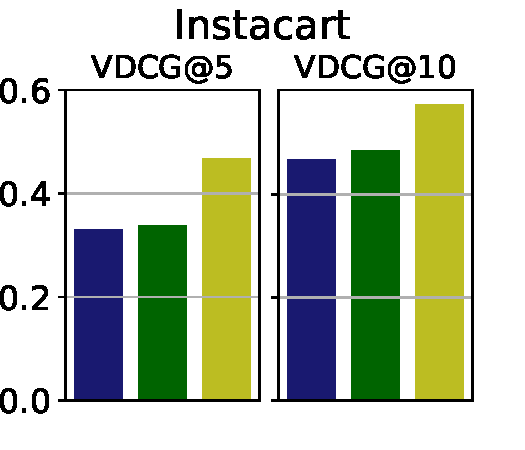
\includegraphics[width=\textwidth]{sections/6_AgentDR/figures/VDCG/vdcg_Instacart.pdf}
    \end{subfigure}
    \hspace{-3mm}
    % \hfill
    \begin{subfigure}{0.3\textwidth}
    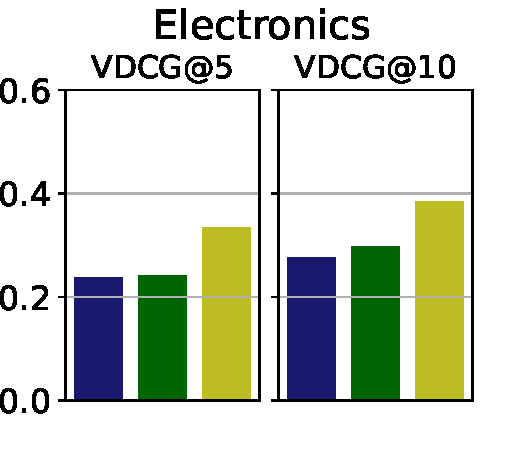
\includegraphics[width=\textwidth]{sections/6_AgentDR/figures/VDCG/vdcg_Electronics.pdf}
    \end{subfigure}
    \hspace{-3mm}
    % \hfill
    \begin{subfigure}{0.3\textwidth}
    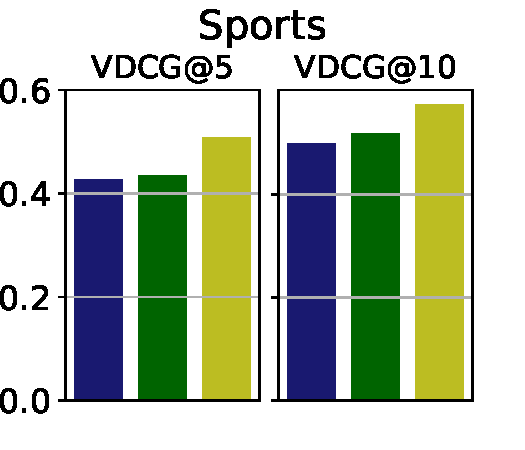
\includegraphics[width=\textwidth]{sections/6_AgentDR/figures/VDCG/vdcg_Sports.pdf}
    \end{subfigure}
    \begin{subfigure}{0.65\textwidth}
    \centering
   \vspace{-2mm}
    
\includegraphics[width=0.9\textwidth]{sections/6_AgentDR/figures/VDCG/bar_legend_horizontal.pdf}
    \end{subfigure}
    \vspace{-4mm}
        \caption{VDCG of AgentDR with and without LLM-based modules.}
  \label{fig_agentdr:vdcg}
\end{figure}


\subsection{RQ3: Aggregation Strategy Analysis}
~\label{sec:ensemble}

\subsubsection{Setup} The ranking comparison in Eq.~\ref{eq_agentdr:rankcmpr} is a simple quantitative reflection mechanism to adjust RecTool weights for personalized tool suitability.  This component is flexible and can be replaced with alternative learning-based ensemble methods.  For instance, we can train a learnable vector $\mathbf{v}\in \mathbb{R}^{1 \times |\mathcal{T}|}$ as adaptive tool weights for all users. This learnable vector is then list-wise multiplied by the ranking score lists $\hat{\mathbf{r}}_\mathcal{T}\in \mathbb{R}^{|\mathcal{T}| \times |\mathcal{I}|}$ of each user to obtain the aggregated ranking score list $\hat{\mathbf{r}}'\in\mathbb{R}^{1\times|\mathcal{I}|}$. Supervised training is performed using ground-truth target items in training set, with a hinge loss as the objective. To integrate this with the original framework, we normalize this $\hat{\mathbf{r}}'$ and $\hat{\mathbf{r}}$ from Eq.~\ref{eq_agentdr:aggrank} and add them as an updated $\hat{\mathbf{r}}$ for the following reranking.

\subsubsection{Results} Table~\ref{tab_agentdr:ensemble} reports the performance of various ensemble strategies, both with and without all LLM-based reasoning modules from AgentDR. The original ranking comparison mechanism and the alternative linear model described above are denoted as \textit{RC} and \textit{LR}, respectively. Additionally, we explore MLP with and without attention mechanisms to capture inter-tool dependencies, as alternatives to the original ranking comparison. These variants are denoted as \textit{Att} and \textit{MLP} in the table. 
The results demonstrate that the proposed reasoning modules consistently provide significant benefits across different ensemble strategies. Although AgentDR equipped with the simplest ranking comparison mechanism already surpasses most baselines in Table~\ref{tab_agentdr:overall}, substituting it with more expressive ensemble methods yields up to a 13.56$\%$ improvement in NDCG. This performance gain comes at the cost of increased computational complexity during backpropagation. Among the evaluated methods, the MLP with an attention mechanism achieves the best overall performance when integrated into AgentDR, which has the the highest number of learnable parameters. We leave the exploration of potential improvement from integrating more advanced ensemble methods in the future work.

\begin{table}
\resizebox{0.65\textwidth}{!}{%
\begin{tabular}{l cc @{\hspace{1.2em}} cc @{\hspace{1.2em}} cc}
\toprule
%Dataset
& \multicolumn{2}{c}{Instacart}
& \multicolumn{2}{c}{Electronics}
& \multicolumn{2}{c}{Sports} \\
\cmidrule(lr){2-3}\cmidrule(lr){4-5}\cmidrule(lr){6-7}
%Metric
& N@10 & N@20
& N@10 & N@20
& N@10 & N@20 \\
\midrule

Ensemble: RC
& 0.0428 & 0.0633
& 0.0765 & 0.0874
& 0.0859 & 0.1009 \\
+ AgentDR
& 0.0701 & 0.0825
& 0.1149 & 0.1227
& 0.1221 & 0.1286 \\
\midrule

Ensemble: LR
& 0.0401 & 0.0638
& 0.0862 & 0.0893
& 0.0950 & 0.1060 \\
+ AgentDR
& \textbf{0.0796} & \textbf{0.0907}
& 0.1136 & 0.1200
& 0.1246 & 0.1297 \\
\midrule

Ensemble: MLP
& 0.0397 & 0.0635
& 0.0754 & 0.0861
& 0.1009 & 0.1056 \\
+ AgentDR
& 0.0747 & 0.0858
& 0.1071 & 0.1166
& 0.1247 & 0.1328 \\
\midrule

Ensemble: Att
& 0.0473 & 0.0692
& 0.0787 & 0.0878
& 0.1000 & 0.1078 \\
+ AgentDR
& 0.0765 & 0.0844
& \textbf{0.1180} & \textbf{0.1260}
& \textbf{0.1247} & \textbf{0.1326} \\
\bottomrule
\end{tabular}%
}
\caption{Ensemble methods with LLM reasoning modules from AgentDR.}
\label{tab_agentdr:ensemble}
\vspace{-3mm}
\end{table}


\subsection{RQ4: Ablation Study}
% To quantify the contribution of each LLM-based module, we compare AgentDR with different modules removed or replaced. 
% For fair comparison, we use the original ranking comparison as quantitative comparison module.
% The ranking comparison is used as quantitative comparison module.
\subsubsection{Tool Comparison and Dual S\&C Reranking}
We investigate the contribution of the proposed tool comparison and dual S\&C reranking modules, denoted as \textit{T} and \textit{Dual S\&C}, respetively. We also explore the effect of replacing dual S\&C by a mutually exclusive substitute or complement reranking based on intent memory of each user, denoted as \textit{S/C}. The general reranking module is excluded from this study. The results are shown in Fig.~\ref{fig_agentdr:ablation}. We observe that tool comparison improves performance in most settings, while it may degrade performance on Instacart. In this dataset, the semantic differences between the grocery food lists recommended by different tools are less pronounced, providing weaker signals for LLM-based tool selection. Moreover, the dual S\&C reranking consistently outperforms reranking based on either substitutes or complements alone across all settings, highlighting the advantage of a more comprehensive reranking strategy.

\begin{figure}[]
    \begin{subfigure}{0.3\textwidth}
    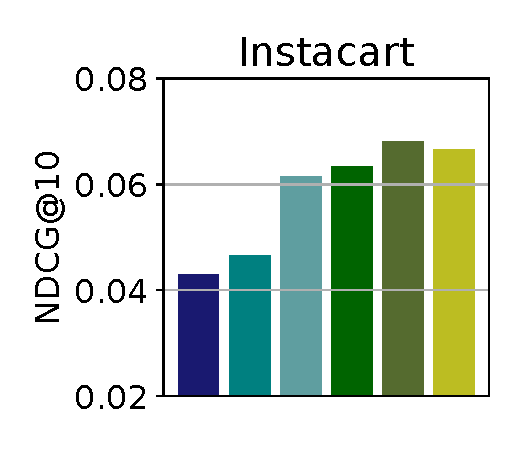
\includegraphics[width=\textwidth]{sections/6_AgentDR/figures/ablation/TDS/TDS_Instacart.pdf}
    \end{subfigure}
    \hspace{-3mm}
    % \hfill
    \begin{subfigure}{0.3\textwidth}
    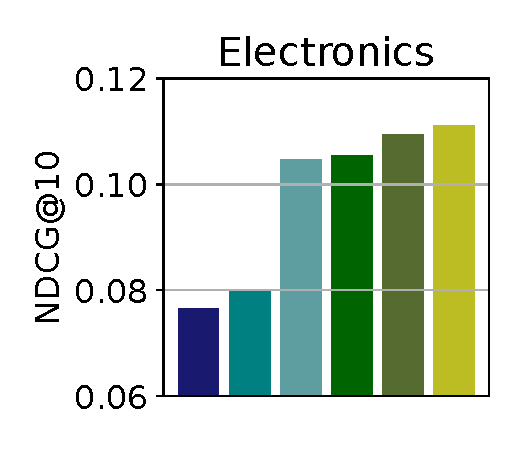
\includegraphics[width=\textwidth]{sections/6_AgentDR/figures/ablation/TDS/TDS_Electronics.pdf}
    \end{subfigure}
    \hspace{-3mm}
    % \hfill
    \begin{subfigure}{0.3\textwidth}
    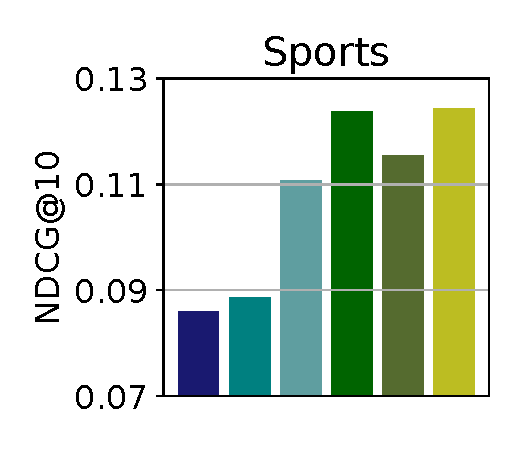
\includegraphics[width=\textwidth]{sections/6_AgentDR/figures/ablation/TDS/TDS_Sports.pdf}
    \end{subfigure}
    \begin{subfigure}{0.75\textwidth}
    \centering
   \vspace{-2mm}
    
\includegraphics[width=\textwidth]{sections/6_AgentDR/figures/ablation/TDS/bar_legend_horizontal.pdf}
    \end{subfigure}
    \vspace{-4mm}
        \caption{Ablation study on comparison and reranking modules in AgentDR.}
  \label{fig_agentdr:ablation}
\end{figure}

\subsubsection{General Reranking}
The general reranking module in Sec.~\ref{sec:genrerank} refines recommendation lists based on summarized user preferences, independent of substitution and complementarity signals. In Table~\ref{tab_agentdr:genrerank}, we compare the performance of AgentDR with and without this module under different reranking settings. The results show that general reranking consistently improves performance in most cases, and all best results across the three datasets are achieved with this module enabled, confirming the importance of general preference signals in complementing intent-specific reasoning. Since the corresponding intent identification module in Eq.~\ref{eq_agentdr:reglearn} accounts for one-third of all inference calls during agent optimization, it can be optionally deactivated to save computational resources in this flexible agent framework, without sacrificing the general preference signals. In such cases, $m_{reg}$ is set as a constant regularization coefficient shared across all users in the dataset.

\begin{table}
\resizebox{0.65\textwidth}{!}{%
\begin{tabular}{l cc @{\hspace{1.2em}} cc @{\hspace{1.2em}} cc}
\toprule
Dataset
& \multicolumn{2}{c}{Instacart}
& \multicolumn{2}{c}{Electronics}
& \multicolumn{2}{c}{Sports} \\
\cmidrule(lr){2-3}\cmidrule(lr){4-5}\cmidrule(lr){6-7}
Metric
& N@10 & N@20
& N@10 & N@20
& N@10 & N@20 \\
\midrule

S/C
& 0.0614 & 0.0740
& 0.1047 & 0.1076
& 0.1107 & 0.1174 \\
+ General
& 0.0676 & 0.0817
& 0.1026 & 0.1120
& 0.1109 & 0.1190 \\
\midrule

T+S/C
& 0.0634 & 0.0794
& 0.1054 & 0.1136
& 0.1238 & 0.1320 \\
+ General
& 0.0626 & 0.0800
& 0.1055 & 0.1149
& \textbf{0.1244} & \textbf{0.1323} \\
\midrule

Dual S\&C
& 0.0682 & 0.0805
& 0.1095 & 0.1174
& 0.1155 & 0.1203 \\
+ General
& 0.0684 & 0.0824
& 0.1050 & 0.1109
& 0.1190 & 0.1238 \\
\midrule

T+Dual S\&C
& 0.0666 & 0.0793
& 0.1112 & 0.1211
& 0.1240 & 0.1307 \\
+ General
& \textbf{0.0701} & \textbf{0.0825}
& \textbf{0.1149} & \textbf{0.1227}
& 0.1221 & 0.1286 \\
\bottomrule
\end{tabular}%
}
\caption{Performance of AgentDR with and without general reranking.}
\label{tab_agentdr:genrerank}
\end{table}


\section{Chapter Summary}
In this chapter, we propose a novel LLM-based agent framework, AgentDR, for full-ranking recommendation. 
It leverages the reasoning capabilities of LLMs to delegate the full-ranking task to multiple recommendation tools in a personalized manner. Furthermore, the commonsense world knowledge of the LLM is utilized to infer user intent regarding substitutes and complements, which is a challenging aspect for traditional models to capture effectively for recommendation enhancement. 
Extensive experiments are conducted with a proposed LLM-based evaluation metric VDCG to evaluate both semantic relevance and ordering correctness of recommendation results. 
Similar to ERLSC, a limitation of this framework is that substitution and complementarity relationships are more prevalent in domains like groceries than in others such as movies or music. 

